\documentclass[a4paper]{jsarticle}
\usepackage[all]{xy}
\usepackage[dvipdfmx]{graphicx}
\usepackage{../math_note, exercise, enumitem}
\renewcommand{\thesection}{Ex7.\arabic{section}}

\newcommand{\coverU}{\mathfrak{U}}
\newcommand{\coverV}{\mathfrak{V}}

\newcommand{\Div}{\operatorname{Div}}
\newcommand{\Cl}{\operatorname{Cl}}
\newcommand{\CaCl}{\operatorname{CaCl}}
\newcommand{\nullCaCl}{\operatorname{CaCl}^{0}}
\newcommand{\Pic}{\operatorname{Pic}}

\begin{document}
    以下での($*$)とは,次のもの:
    \begin{itemize}
        \item integral,
        \item separated,
        \item noetherian, and
        \item regular in codimention one.
    \end{itemize}

    また,($\dagger$)は次のもの:
    $X$ :: noetherian scheme, 
    $\shS$ :: graded $\shO_X$-algebra
    となっている.
    また,$d \in \Z, d \geq 0$について,
    $\shS_d$ :: homogeneous part of $\shS$を$U \mapsto \shS(U)_d$.
    $X,\shS$は次をすべて満たす.
    \begin{itemize}
        \item $\shS$ :: quasi-coherent.
        \item $\shS=\bigoplus_{d \geq 0} \shS_d$.
        \item $\shS_0=\shO_X$.
        \item $\shS_1$ :: coherent $\shO_X$-module.
        \item $\shS$ :: locally generated by $\shS_1$ as $\shO_X$-algebra.
    \end{itemize}

\section{Surjective Mophism between Invertible Sheaves is Isomorphic.} %% Ex7.1 
    $X$ :: locally ringed space,
    $\shL, \shM$ :: invertible sheaves on $X$,
    $f: \shL \to \shM$ :: surjective mophism,
    とする.
    
    \paragraph{Proof 1.}
    任意の点$x \in X$をとり,$A=\shO_{X,x}$とおく.
    $f_x: \shL_x \to \shM_x$は同型写像を合成することで
    $\phi: A \to A$ :: surjective $A$-morphismと同一視出来る.
    $\phi$ :: surjectiveより,
    $\phi(\alpha)=1 \in A$となる$\alpha \in A$がとれる.
    また$\phi$は$A$-module morphismだから,$\alpha \phi(1)=1$.
    そこで$\psi: A \to A$を$a \mapsto \alpha a$と定義すれば,
    これが$\phi$の逆写像になる.
    よって$\phi, f_x$は同型.
    Prop1.1から,$f$ :: iso.

    \paragraph{Proof 2.}
    Matsumura, Thm2.4から分かる.
    これはNAK (or Nakayama's Lemma)からの帰結である.

    \begin{Remark}
        $k(x)$ :: residue fieldと
        $f_x: \shL_x \to \shM_x$をテンソルすると,
        $f_x \otimes \id{k(x)}$ :: surjective $k(x)$-module morphismが得られる.
        よって$\ker (f_x \otimes \id{k(x)})=0$.
        しかし,ここからNAKをつかって$\ker f_x=0$を導くことは出来ない.
        $k(x)$がflat $\shO_{X,x}$-moduleでなく,
        したがって$\ker (f_x \otimes \id{k(x)})$と$(\ker f_x) \otimes k(x)$の間に同型があることが
        言えないからである.
        このことはflat $\implies$ torsion-freeに気をつければすぐに分かる.
        同様の議論が$f_x$ :: injective(と$\coker f_x$)の場合に出来ることにも気づくが,
        このときは$\Z_2 \to \Z_2; 1 \mapsto 3$という反例がある.
    \end{Remark}

\section{Two Sets of Global Generators and Corresponding Morphisms.} %% Ex7.2 
    $k$ :: field,
    $X$ :: scheme /$k$,
    $\shL$ :: invertible sheaf on $X$,
    $S=\{s_0,\dots,s_m\}, T=\{t_0,\dots,t_n\}$ :: global generators of $\shL$.
    とする.
    ここで$S,T$は
    同じ線形(部分)空間$V \subseteq \Gamma(X, \shL)$を張るとする.
    また$n \leq m, d=\dim_k V$とする.

    $S,T$からそれぞれThm7.1のように定まるmorphismを$\phi_S, \phi_T$とする.
    $\phi_S$が次のように分解できることを示す.
    \[
        \xymatrix
        {
            X \ar@/_20pt/[rrrr]_-{\phi_S}\ar[r]^-{\phi_T}&
                \im \phi_T \ar@{^{(}->}[r]& \proj^m-L \ar[r]^-{\pi}&
                    \proj^n \ar[r]^-{\alpha}& \proj^n
        }
    \]
    ここで$\pi, \alpha$はそれぞれlinear projectionとautomorphismである.

    $X \to \proj^n$のmorphismを考えることは,
    $k[y_0,\dots, y_n]$の元$y_0,\dots,_n$の変換を考えることと同じである.
    これはThm7.1の証明を観察すれば分かる.
    二つの$k$-linear mapは$\phi_S^*, \phi_T^*$はそれぞれ,
    $y_i \mapsto s_i (i=0,\dots,n)$,
    $y_i \mapsto t_i (i=0,\dots,m)$で定まっている.
    したがって問題は,
    $t_0,\dots,t_m$を$s_0,\dots,s_n$へ
    変換するprojectionとautomorphismをつくる問題,
    と言い換えられる.

    今,次のような$(m+1) \times (n+1)$行列$Q$が存在する.
    \[
        \tatev{ s_0 \\ \vdots \\ s_n }
        =Q \tatev{ t_0 \\ \vdots \\ t_m }.
    \]
    $S,T$が$V$の生成系であることから$\rank Q=\dim V=:d$.
    $Q$は基本行列をいくつもかける(あるいは基本変形を繰り返し行う)ことにより,
    次の形に分解できる.
    \[
        Q=L P_{d} R~~
        \mwhere~ L \in PGL(m,k), R \in PGL(n,k)
    \]
    ただし行列$P_r ~(r=1,\dots,n+1)$は$r \times r$-identity matrix $I_r$をもちいて
    $P_{r}=
    \begin{bmatrix}
        I_r & 0 \\
        0 & 0
    \end{bmatrix}$
    と定義される行列である.
    (TODO: $P_{d}$を$P_{n+1}$に交換しても問題ない?)
    $L, P_{n+1}, R$が誘導するmorphismをそれぞれ$\beta, \tilde{\pi} ,\alpha$とすれば,
    $\alpha, \beta$はautomorphismであり,
    $\tilde{\pi}$はprojectionである.
    \[
        \xymatrix
        {
            \proj^m \ar[r]^-{\beta}& \proj^m
            \ar@{^{(}->}[r]^-{i}& \proj^m-L
            \ar[r]^-{\tilde{\pi}}& \proj^n
            \ar[r]^-{\alpha}& \proj^n
        }
    \]
    求める写像はこの$\alpha$と,$\pi=\beta \circ i \circ \tilde{\pi}$である.
    また,$L=\zerosp(y_0,\dots,y_n) \subseteq \proj^m$の次元は$m-(n+1)$である.

\section{Morphism of $\proj^n \to \proj^m$ can be Decomposed into Common Ones.} %% Ex7.3
    $\phi: \proj^n_k \to \proj^m_k$を考える.
    $\shO_{\proj^m}(1), \shO_{\proj^n}(1)$
     :: invertible sheaves
    のglobal generatorをそれぞれ
    $\{x_0,\dots,x_m\}, \{y_0,\dots,y_n\}$
    とする.

    \subsection{$\im \phi=pt$ or $m \geq n$ and $\dim \im \phi=n$.}
%    $\eta: \Gamma(\proj^m, \shO_{\proj^m}(1)) \to \Gamma(\proj^m, \phi^* \phi_* (\shO_{\proj^m}(1)))$を
%    adjoint pair $\phi^* \dashv \phi_*$のunitから得られる写像とする.
%    これが本文中で$\phi^*$と表記されているものである
    $s_i=\phi^*(x_i)~(i=0,\dots,m)$とおくと,
    $s_0,\dots,s_m$は$\shL:=\phi^*(\shO_{\proj^m}(1))$のglobal generatorである.
    $\shL$は$\proj^n$上のinvertible sheafだから,
    Cor6.17より,$\shL \iso \shO_{\proj^n}(d)$となる$d \in \Z$が存在する.
    Example7.8.3同様,$\shO_{\proj^n}(d)$は$|d|$次斉次単項式で生成される.

    \paragraph{$m<n \implies \dim \im \phi=0$.}
    \paragraph{$m \geq n \implies \dim \im \phi=n$.}

\section{If $X$ Admits an Ample Invertible Sheaf, then $X$ is Separated.} %% Ex7.4

    \subsection{Assumption of Thm7.6 $\implies$ $X$ :: separated.}
    $A$ :: noetherian ring,
    $X$ :: scheme of finite type /$A$とする.
    $\shL$ :: ample invertible sheaf on $X$が存在したとする.
    Thm7.6の証明(特にp.155の第二段落)から次が分かる:
    十分大きい$n>0$をとると,
    $s_1,\dots,s_k \in \Gamma(X,\shL^n)$が存在し,
    $X_i=X_{s_i}$
    \footnote
    {
        $X_{s_i}$は
        $\{P \in X \mid (s_i)_P \not \in \I{m}_P \shL^n_{P} \}$
        で定義される開集合.
        cf. Ex2.16.
    }
    はaffine open coverを成す.
    $U_i=V^c(x_i)$とすると,これもaffine open cover.
    Thm7.6において引き続いて構成されるimmertion $\phi: X \to \proj^N_A$は,
    (証明の最終段落から)$\phi^{-1}(U_i)=X_i$を満たす.
    $U_i, X_i$は共にaffineであるから,
    $\phi|_{X_i}: X_i \to U_i$はseparated (Prop4.1).
    Cor4.6fより$\phi: X \to \proj^N_A$はseparated.
    $\proj^N_A \to \Spec A$はprojective (Example4.8.1)なのでsperated.
    よってseparated morphismの合成$X \to \proj^N_A \to \Spec A$も
    separatedである.

    \subsection{There is No Ample Invertible Sheaf on 
        \protect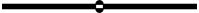
\includegraphics[width=2.5cm]{./images/affine_with_doubled_origin2.eps} / a field $k$.}
    $k$ :: field,
    $X$ :: affine with doubled origin /$k$とする.
    より詳細に,$X$は$X_1=\Spec k[x], X_2=\Spec k[y]$を
    $U_1=X_1-\{O_1\}, U_2=X_2-\{O_2\}$で貼りあわせたものとする.
    ただし$O_1 \in X_1,O_2 \in X_2$は原点である.
    $X_i, U_i, O_i ~~(i=1,2)$はすべて$X$の部分集合とみなす.
    $X$ :: noetherian integral schemeは明らか.
    Example 6.3.1, Cor 6.16より,$\Pic X_1, \Pic X_2=0$.

    まず$\Pic X$を計算する.
    これには$k[x], k[y]$がUFDであることを用いる.
    $X$ :: integralより$\Pic X \iso \CaCl X$ (Prop6.15).
    なので$\CaCl X$を計算する.
    Example 4.0.1にある$\shO_X$の定義から計算すると,
    $K_X$ :: function field of $X$は次のように書ける.
    \[ K_X=\{ (f,g) \in k(x) \times k(y) \mid \phi(f|_{U_1 \cap U_2})=g|_{U_1 \cap U_2}. \} \]
    ただし$\phi$は$x \mapsto y$で定まる同型である.
    $O_1$に対応するイデアルは単項イデアル $(x)$であるから,
    $f$は$x^n h$の様に書くことが出来る.
    この$h$は$O_1$で零点も極も持たない元,
    すなわち$\shO_{X_1, O_1}=k[x]_{(x)}$の単元である.
    $g$についても同様であるから,
    結局次のように成る.
    \[
        K_X=
        \{
            (x^n, y^n) \cdot (f, g)
            \mid
            n \in \Z, 
            ( f,g) \in \shO_{X_1, O_1}^* \times \shO_{X_2, O_2}^*,
            \phi(f|_{U_1 \cap U_2})=g|_{U_1 \cap U_2}.
        \}
    \]
    $K_X^*$の元がprincipal divisorだから,
    $\CaCl X \iso \{ (x^n, y^n) \in k(x) \times k(y) \mid n \in \Z \} \iso \Z$.

\section{Ample and Very Ample are Inherted by Tensor Products.} %% Ex7.5 

\section{The Riemann-Roch Problem.} %% Ex7.6 

\section{Some Rational Surfaces.} %% Ex7.7 

\section{Sections of $\pi: \P(\shE) \to X$
    $\leftrightarrow$ Quotient Invertible Sheaves of $\shE$.} %% Ex7.8 

\section{ } %% Ex7.9 

\section{$P^n$-Bundles Over a Scheme.} %% Ex7.10 

\section{Different Sheaves of Ideals can Give Rise to Isomorphic Blown Up Schemes.} %% Ex7.11 

\section{ } %% Ex7.12 

\section{* A Complete Nonprojective Variety.} %% Ex7.13 

\section{ } %% Ex7.14 


\end{document}
